\section{Method}

The obstacle for generating an interlocking pattern for FDM 3D printing is satisfying the semi-continuous extrusion constraint.
We propose a geometry consisting of parallel horizontal beams of alternating material for even layers and the same pattern but rotated by some angle for odd layers, 
so that it connects the beams of the even layers and thusly interlocks the other material.
This design ensures semi-continuous extrusion in two ways:
\begin{itemize*}
	\item the geometry contains beams connected to the outline of the shape such that the outer wall is a continuous line for both the shape and the beams
	\item the geometry contains cross beams which are long and horizontal, so that the toolpaths to fill them are as such as well.
\end{itemize*}

\tim{Show that this geometry is high genus and interlocking.}

\tim{Show picture of the general idea.}

The proposed geometry had several design variables and it might be optimized for several loading conditions.
For simplicity we will consider only tensile forces perpendicular to the interface between the two bodies.
Design variables include beam widths and heights for either material.
Also the horizontal orientation of the pattern w.r.t. a vertical interface is of interest.
Rotating our pattern about a horizontal axis is not a design variable, because then the geometry would violate the continuity constraint .

Let's consider a vertical interface, 
i.e. the two bodies lie horizontally next to each other.
The tensile force will then be applied horizontally orthogonal to the interface.
Because this combination of interface and tensile load is symmetrical, 
we only consider two orientations of the interlocking pattern:
\begin{description}
	\item[Straight] even beams (`cross beams') are aligned parallel to the interface and odd beams (`fingers') are perpendicular
	\item[Diagonal] even beams and odd beams (both `fingers') are at equal and opposite angles w.r.t. the interface.
\end{description}






\subsection{Straight Orientation}

\begin{figure}
	\centering
	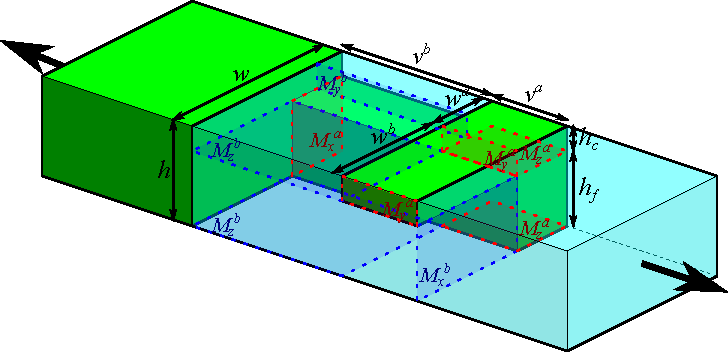
\includegraphics[width=\columnwidth]{sources/method/straight_model_v2.pdf}
	\caption{
		One straight unit cell connecting material $a$ (left) to material $b$ (right).
		Failure can happen along the fingers ($M_x$), along the cross beams ($M_y$) or at the interface between the two ($M_z$) for either material.}
	\label{fig:failure_modes}
\end{figure}




\begin{table}
	\centering
	\caption{Material properties according to Ultimaker technical data sheets. \todo{Starred* data will have to be rechecked.}}
	\label{tab:mat_props}
	\begin{tabular}{lrrrl}
		& PLA & PP & TPU & \\
		$E$ & 2797 & 302 & 67 & \si{\mega\pascal} \\
		$E_z$ & 2696 & 262 & 56 & \si{\mega\pascal} \\
		$\sigma_\text{yield}$ & 47 & 10.5 & - & \si{\mega\pascal} \\
		$\sigma_\text{z,yield}$ & 33 & 9.0* & - & \si{\mega\pascal} \\
		$\epsilon_\text{yield}$ & 3.5 & 29 & - & \si{\percent} \\
		$\epsilon_\text{z,yield}$ & 2.6 & 25* & - & \si{\percent} \\
		$\sigma_\text{break}$ & 31 & 9.4 & 38 & \si{\mega\pascal} \\
		$\sigma_\text{z,break}$ & 32 & 7.8* & 6.4 & \si{\mega\pascal} \\
		$\epsilon_\text{break}$ & 8.2 & 70* & $>700$ & \si{\percent} \\
		$\epsilon_\text{z,break}$ & 3.1 & 50* & 82 & \si{\percent} \\
	\end{tabular}
\end{table}



If we would only consider the size of the beams of the two materials,
the optimal ratio would be when both materials would fail at the same time:
$
A^\text{PP} / A^\text{PLA} = \sigma^\text{PLA}_\text{break} / \sigma^\text{PP}_\text{yield}  \approx 4.3
$.
See \cref{tab:mat_props}.
For example, if the beams are the same height and the PLA beams are the minimum of twice the line width of the default printing profile, \SI{0.7}{\milli\meter}, 
then the PP beams should be \SI{3.0}{\milli\meter}.

However, such an analysis is oversimplified, because it reduces the design variables to only two,
while in fact we have six.
\Cref{fig:failure_modes} shows one unit cell with the variables for material $a$ and $b$.


Without loss of generality let's assume material $a$ is TODO

When considering the structure failure can happen in different ways.
\Cref{fig:failure_modes} shows the types of failure mode.
Because of the high genus interlocking, some of these failure modes are not enough to break the structure apart.
It is specifically only the $M_y$ failure modes which still require any of the other failures to happen for the two materials not to be interlocking any more.
We can therefore ignore the $M_y$ failure modes and concentrate only on the $M_x$ and $M_z$ failure modes.

$M_y^a$ will always occur before $M_y^b$ happens.

\tim{Put more emphasis on the point that we can ignore failure mode $M_y$.}



\subsection{Optimal Multi-stage Geometry}

\tim{Refactor this section to something shorter, because we found out that $N>1$ only gives worse performance.}

Let's consider a PLA finger which crosses $N$ beams, which is allowed to vary in width.
See \cref{fig:force_distribution}.
In case one segment would have a higher stress than the others then that one would be the weakest link, so in the optimal structure all segments have the same stress $\sigma$.
However, when the two materials are different it is not possible to optimize the structure such that both links will break at the same time.
Since the links of the fingers are (inter)locked at either end the elongation of the link will be shared among both materials, so the material with the lowest value for elongation at break will always be the link that breaks first.
We therefore set the stress along all links with the material with the lower elongation at break at the yield stress, while setting only the stress of the base link of the other material at its respective yield stress;
the stresses of the other links will be lower, because they are constrained: 

\begin{align}
	\sigma^a_x = \sigma^a_\text{yield} \label{eq:stress_equality}
\end{align}

Let's assume, without loss of generality, that material $a$ yields (or breaks) at a lower strain value
and that $a$ yields before $b$ yields (?), i.e. $\sigma^a_{\text{ yield}} < \sigma^b_{\text{ yield}} \nicefrac{E^a}{E^b}$.
Then the total strain when the link fails is determined by $a$.

From \cref{fig:force_distribution} we can see that the widths of opposite finger segments add up to the cell width $w$ and that the tension forces in the links add up.
The forces transferred between the fingers via the cross beams cover the difference in forces between two consecutive finger segments.
This equilibrium condition means that the boundary between two cross-beams is in a resting position.
These give rise to the following formulae:

\begin{align}
	w &= w_x^a + w_{N+1-x}^b \label{eq:width_formula} \\
	F_1^a &= F_1^b = F_x^a + F_{N+2-x}^b  \label{eq:forces_formula}
\end{align}

\begin{figure}
	\centering
	\begin{subfigure}{\columnwidth}
		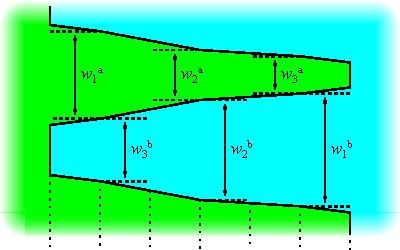
\includegraphics[width=\columnwidth]{sources/method/varying_width_fingers.pdf}
		\caption{Top view}
	\end{subfigure}
	\begin{subfigure}{\columnwidth}
		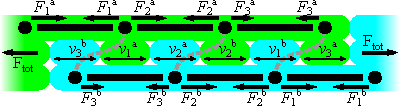
\includegraphics[width=\columnwidth]{sources/method/stress_distribution.pdf}
		\caption{Side view (schematic)}
	\end{subfigure}
	\caption{Tension forces in the links of fingers with varying width. The effective width of a link equals the smallest width along the link.}
	\label{fig:force_distribution}
\end{figure}


Given an extension $\epsilon$ of a link consisting of two parallel beams $a$ and $b$ which are connected at the ends,
the distribution of forces depends on the ratio in Young's moduli and the ratio in cross section:
\begin{align}
	%E &\equiv \frac{\sigma}{\epsilon} \\
	%\sigma &= E \epsilon \\
	%\frac{\sigma^a}{\sigma^b} &=  \frac{E^a \epsilon}{E^b \epsilon} 
	%= \frac{E^a}{E^b}  \\
	%\\
	%\sigma &\equiv \frac{F}{A} \\
	% F &= \sigma A = E \epsilon hw \\
	%\frac{F^a}{F^b} &= \frac{E^a \epsilon h_\text{f} w^a}{E^b \epsilon h_\text{f} w^b}
	%= \frac{E^a w^a}{E^b w^b} \\
	F^b &= F^a \frac{E^b}{E^a} \frac{w^b}{w^a} \label{eq:double_beam_force_distribution}
\end{align}












\subsection{Optimal Varying Finger Width Derivation}

Using \crefrange{eq:stress_equality}{eq:double_beam_force_distribution} we can derive a formula for the widths of material $b$:

\iffalse
In general, without assuming equal stresses in a:
\begin{align*}
	%\sigma_x^m &= \frac{F_x^m}{w_x^m h}\\
	F_1^a &= F_1^b % = F_x^a + F^a_x \frac{E^b}{E^a} \frac{w^b_{N+2-x}}{w^a_x} \\
	= F_x^a \left( 1 + \frac{E^b}{E^a} \frac{w^b_{N+2-x}}{w^a_x} \right) \\
	% w_1^a h_\text{f} \sigma_1^a &= w_1^b h_\text{f} \sigma_1^b = w_x^a h_\text{f} \sigma_x^a + w_{N+2-x}^b h_\text{f} \sigma_{N+2-x}^b \\
	w_1^a \sigma_1^a &= w_1^b \sigma_1^b = w_x^a \sigma_x^a \left( 1 + \frac{E^b}{E^a} \frac{w^b_{N+2-x}}{w^a_x} \right) \\
	%&= w_x^a \sigma_x^a + w_x^a \sigma_x^a \frac{E^b}{E^a} \frac{w^b_{N+2-x}}{w^a_x} \\
	&= w_x^a \sigma_x^a + \sigma_x^a \frac{E^b}{E^a} w^b_{N+2-x} \\
	w_1^a &= w_x^a \frac{\sigma_x^a}{\sigma_1^a} + \frac{\sigma_x^a}{\sigma_1^a} \frac{E^b}{E^a} w^b_{N+2-x} \\
	%w_1^a \sigma_1^a &= w_1^b \sigma_1^b = w_x^a \sigma_x^a + w_{N+2-x}^b \sigma_{N+2-x}^b \\
	w_N^b &= w - w_1^a =  w_x^a + w_{N+1-x}^b  -  w_x^a \frac{\sigma_x^a}{\sigma_1^a} - \frac{\sigma_x^a}{\sigma_1^a} \frac{E^b}{E^a} w^b_{N+2-x} \\
	&= w_x^a \left( 1 - \frac{\sigma_x^a}{\sigma_1^a} \right) + w_{N+1-x}^b - \frac{\sigma_x^a}{\sigma_1^a} \frac{E^b}{E^a} w^b_{N+2-x} \\
\end{align*}

If material $a$ will fail first then the optimal structure has the same stress for material $a$ in each beam, i.e. $\sigma_x^a = \sigma_1^a$.

\fi


\begin{align}
	%w_N^b &= w_{N+1-x}^b - \frac{E^b}{E^a} w^b_{N+2-x} \\
	%w_N^b &= w_{x}^b - \frac{E^b}{E^a} w^b_{x+1} \\
	w_{x}^b &= w_N^b + \frac{E^b}{E^a} w^b_{x+1} \\
	%\\
	%% x = N - 1
	%w_{N-1}^b &= w_N^b + \frac{E^b}{E^a} w^b_{N} \\
	%&= w_N^b \left( 1 + \frac{E^b}{E^a} \right) \\
	%\\
	%% x = N - 2
	%w_{N-2}^b &= w_N^b + \frac{E^b}{E^a} w^b_{N-1} \\
	%&= w_N^b + \frac{E^b}{E^a} w_N^b \left( 1 + \frac{E^b}{E^a} \right) \\
	%&= w_N^b \left( 1 + \frac{E^b}{E^a} \left( 1 + \frac{E^b}{E^a} \right) \right) \\
	%&= w_N^b \left( 1 + \frac{E^b}{E^a} + \left(\frac{E^b}{E^a} \right)^2 \right) \right) \\
	%\\
	%% x = N - 3
	%w_{N-3}^b &= w_N^b + \frac{E^b}{E^a} w^b_{N-2} \\
	%&= w_N^b + \frac{E^b}{E^a} w_N^b \left( 1 + \frac{E^b}{E^a} \left( 1 + \frac{E^b}{E^a} \right) \right) \\
	%&= w_N^b \left( 1 + \frac{E^b}{E^a} \left( 1 + \frac{E^b}{E^a} \left( 1 + \frac{E^b}{E^a} \right) \right) \right) \\
	%&= w_N^b \left( 1 + \frac{E^b}{E^a} + \left(\frac{E^b}{E^a} \right)^2  + \left(\frac{E^b}{E^a} \right)^3 \right) \right) \\
	%\\
	%\dots \\
	%w^b_{N-x} &= w^b_N \sum\limits_{i=0}^x \left(\frac{E^b}{E^a}\right)^i \\
	w^b_{x} &= w^b_N \sum\limits_{i=0}^{N-x} \left(\frac{E^b}{E^a}\right)^i \label{eq:widths_b}
\end{align}

We will optimize the structure such that material $b$ will break at the base at the same point as material $a$ break anywhere along the chain, i.e. $\sigma^b_1 = \sigma^b_\text{yield}$ and $\sigma^a  = \sigma^a_\text{yield}$.
Using \cref{eq:forces_formula} we can then derive the width of the first link of material $a$ and from that one we can derive the rest using \cref{eq:width_formula}:

\begin{align}
	%\sigma_x^m &= \frac{F_x^m}{w_x^m h}\\
	%h_\text{f} w_1^a &= \frac{F_1^a}{\sigma^a} \\
	%&= \frac{F_1^b}{\sigma_1^b} \frac{\sigma^b_\text{yield}}{\sigma^a_\text{yield}}\\
	%&= w_1^b h_\text{f} \frac{\sigma^b_\text{yield}}{\sigma^a_\text{yield}}\\
	w_1^a &= w_1^b \frac{\sigma^b_\text{yield}}{\sigma^a_\text{yield}} \label{eq:width_a_1} \\
	%\end{align}
	%\begin{align}
	%w &= w^a_1 + w^b_N \\
	%&= w_1^b \frac{\sigma^b_\text{yield}}{\sigma^a_\text{yield}} + w^b_N \\
	%&= w^b_N \sum\limits_{i=0}^{N-1} \left(\frac{E^b}{E^a}\right)^i \frac{\sigma^b_\text{yield}}{\sigma^a_\text{yield}} + w^b_N \\
	%&= w^b_N \left( \frac{\sigma^b_\text{yield}}{\sigma^a_\text{yield}} \sum\limits_{i=0}^{N-1} \left(\frac{E^b}{E^a}\right)^i  + 1 \right) \\
	%\\
	%w^a_x &= w - w^b_{N+1-x} \\
	%&= w^b_N \left( \frac{\sigma^b_\text{yield}}{\sigma^a_\text{yield}} \sum\limits_{i=0}^{N-1} \left(\frac{E^b}{E^a}\right)^i  + 1 \right) - \left( w^b_N \sum\limits_{i=0}^{x-1} \left(\frac{E^b}{E^a}\right)^i  \right) \\
	w^a_x &= w^b_N \left( 1 + \frac{\sigma^b_\text{yield}}{\sigma^a_\text{yield}} \sum\limits_{i=0}^{N-1} \left(\frac{E^b}{E^a}\right)^i  - \sum\limits_{i=0}^{x-1} \left(\frac{E^b}{E^a}\right)^i  \right) \label{eq:widths_a}
\end{align}

We conclude that for any given $N$ and given material properties the widths depend linearly on each other.
This means we can scale up the widths such that the smallest width is still manufacturable,
which is the tip of the finger of material $a$:
$w^a_N = w_\text{min}$







\subsubsection{Optimal Cross Beam Dimensions}
So far we have optimized the widths of the fingers against failure mode M1.
Let's now consider the required widths of the cross-beams to prevent failure mode M2.
See \cref{fig:failure_modes}.
The shear stress enacted on the cross-beams equals the force which is transferred between the fingers through the cross-beams.


\begin{align}
	F^{b \text{,beam}}_x &= F^{a \text{,beam}}_{N+1-x} \label{eq:beam_force_equality} \\
	F^{a \text{,beam}}_N &= F^a_N \label{eq:beam_force_N}\\
	F^{a \text{,beam}}_x &= F^a_x - F^a_{x+1} \label{eq:beam_force_transfer}
\end{align}

Using \cref{eq:stress_equality} and \cref{eq:widths_a} we can then derive:

\begin{align}
	F^{a \text{,beam}}_x 
	%&= \sigma^a_x h_\text{f} w^a_x - \sigma^a_{x+1} h_\text{f} w^a_{x+1} \\
	%&= \sigma^a_\text{yield} h_\text{f} \left( w^a_x - w^a_{x+1} \right) \\
	%&= \sigma^a_\text{yield} h_\text{f} \left( w - w^b_N \sum\limits_{i=0}^{N-x} \left(\frac{E^b}{E^a}\right)^i - w + w^b_N \sum\limits_{i=0}^{N-x-1} \left(\frac{E^b}{E^a}\right)^i \right) \\
	&= \sigma^a_\text{yield} h_\text{f} w^b_N \left(\frac{E^b}{E^a}\right)^{N-x} \label{eq:beam_forces}
\end{align}

Note that for failure mode M2 and M3 the material needs to break in two places, so the effective area is twice as big.
So the cross beams of material $a$ would shear-break when
\begin{align*}
	\frac{F^{a \text{,beam}}_x }{2 v^a_x  h_\text{c}} &= \tau^a \\
	%2 v^a_x  h_\text{c} &= \frac{ F^{a \text{,beam}}_x }{\tau^a} \\
	%v^a_x &= \frac{ F^{a \text{,beam}}_x }{2 \tau^a h_\text{c}} \\
	%\\
	v^a_N
	%&= \frac{ F^a_N }{2 \tau^a h_\text{c}} \\
	%&= \frac{ \sigma^a_\text{yield} w^a_N h_\text{f} }{2 \tau^a h_\text{c} } \\
	&= \frac12 \frac{ \sigma^a_\text{yield}}{\tau^a} \frac{ h_\text{f} }{  h_\text{c} } w^a_N  \\
	v^b_N
	&= \frac12 \frac{ \sigma^a_\text{yield}}{\tau^b} \frac{ h_\text{f} }{  h_\text{c} } w^b_N  \\
	%\\
	%&= \frac{  \sigma^a_\text{yield} h_\text{f} w^b_N \left(\nicefrac{E^b}{E^a}\right)^{N-x}  }{2 \tau^a h_\text{c}} \\
	v^a_x &=  \frac12 \frac{\sigma^a_\text{yield}}{\tau^a} \frac{h_\text{f}}{h_\text{c} } w^b_N \left(\frac{E^b}{E^a}\right)^{N-x}   \\
	%\tau^a &\approx \nicefrac38 \sigma^a_\text{yield} \\ 
	%v^a_x &\approx  \nicefrac83 \frac{h_\text{f}}{h_\text{c} } w^b_N \left(\frac{E^b}{E^a}\right)^{N-x}   \\
	v^b_x
	%&= \frac12 \frac{ F^{b \text{,beam}}_x }{\tau^b h_\text{c}} \\
	&=  \frac12 \frac{ \sigma^a_\text{yield} }{\tau^b } \frac{ h_\text{f}  }{h_\text{c}}   w^b_N \left(\frac{E^b}{E^a}\right)^{x-1} \\
\end{align*}

We conclude that, given constant $N$ and material properties,
the widths of the cross-beams depend linearly on the ratio between beam heights and the finger widths.
Depending on the ratio we will set either $h_\text{c} = h_\text{min}$ or $h_\text{f} = h_\text{min}$,
where $h_\text{min}$ is the manufacturing layer thickness.

One should take care to avoid situations where the cross beam widths are less than the minimum manufacturable width.






\subsubsection{Shearing requirement}
If the height of the total pattern becomes too high the stresses will concentrate along the interface between the fingers and the cross beams.
Such would be the case for failure mode M3.
See \cref{fig:failure_modes}.
The total height $h$ of the pattern should therefore be limited:


\begin{align*}
	\frac{F^{a \text{,beam}}_x }{2w^a_x v^a_x} &< \tau^a \\
	%\frac{F^{a \text{,beam}}_x }{ \tau^a} &< 2 w^a_x v^a_x \\
	%\frac{F^{a \text{,beam}}_x }{ \tau^a} &< 2 w^a_x \frac{ F^{a \text{,beam}}_x }{\tau^a h_\text{c}} \\
	h_\text{c} &< 2 w^a_x  \\
\end{align*}
%(The contact area between a finger and the beam above and the beam below is given by $2 w^a_x v^a_x$ because it's the same on top of the finger as on the bottom.)

TODO: actually the area of the failure mode is less, because of the varying width beams.

Since this holds for all widths, we only need to look at the link with the smallest width:
\begin{align*}
	h_\text{c} &< 2 w^a_N \\
	%h_\text{c} &< 2 w^b_N \left( 1 + \frac{\sigma^b_\text{yield}}{\sigma^a_\text{yield}} \sum\limits_{i=0}^{N-1} \left(\frac{E^b}{E^a}\right)^i  - \sum\limits_{i=0}^{N-1} \left(\frac{E^b}{E^a}\right)^i  \right) \\
	%h_\text{c} &< 2 w^b_N \left( 1 + \left( \frac{\sigma^b_\text{yield}}{\sigma^a_\text{yield}} - 1 \right)     \sum\limits_{i=0}^{N-1} \left(\frac{E^b}{E^a}\right)^i   \right) \\
\end{align*}

Likewise for material $b$, but since that material is less stiff we know that $w^a_N < w^b_N$, so this requirement is redundant.



The analytical approach presented here depends on some simplifications

Should we use $\nicefrac{\sigma_\text{yield} }{ \epsilon_\text{yield} }$ instead of the Young's modulus $E$?

TODO: take into account that the Z shear and tensile forces are different!



\subsection{Optimization}
The optimal structure can withstand the highest forces.
We want to maximize the effective ultimate stress, while keeping the structure as small as possible.

\begin{align}
	& \max \frac{F^m_1}{w \left( h_\text{f} + h_\text{c} \right) } \\
	& \min h_\text{f} + h_\text{c} \\
	& \min w \\
	\text{subject to} & \nonumber \\
	w^m_x &\ge w_\text{min}^m \\
	h_\text{f} &\ge h_\text{min} \\
	h_\text{c} &\ge h_\text{min} \\
	\frac{ F^m_x }{ w^m_x h_\text{f} } &\le \sigma^m_\text{yield} \\
	\frac{ F^m_x - F^m_{x+1} \cdot (x < N ?) }{ 2 v^m_x h_\text{c}} &\le \tau^m \\
	\frac{ F^m_x - F^m_{x+1} \cdot (x < N ?) }{ 2 v^m_x w^m_x } &\le \tau^m_\text{Z} \\
	w &= w_x^a + w_{N+1-x}^b \\
	F_1^a &= F_1^b = F_x^a + F_{N+2-x}^b  \\
	F^b_x &= F^a_{N+2-x} \frac{E^b}{E^a} \frac{w^b_x}{w^a_{N+2-x}} \text{ for } x \ge 2 \\
	\nonumber \\
	F^m_x &= \sigma^m_x w^m_x h_\text{f} \\
\end{align}

Where
\begin{align*}
	m &\in \{a, b\} \\
	1 &\le x \le N \\
\end{align*}


In order to be able to solve this optimization problem we need to introduce more constraints.

If we add a constraint on the total length $\sum v^a_x + \sum v^b_x$ then $N=1$ is always optimal.


\subsubsection{Simple Straight Case}
Let's consider the case for $N=1$.
In that case we only have the following design variables: $w^a, w^b, v^a, v^b, h_\text{f}, h_\text{c}$.
Here we simplify the notation in order to reflect the more simple scenario.
The optimization then consists of the following:

\begin{align}
	& \max \frac{F}{\left( w^a + w^b \right) \left( h_\text{f} + h_\text{c} \right) } \\
	\text{subject to} & \nonumber \\
	w^m &\ge w_\text{min}^m \\
	v^m &\ge v_\text{min}^m \\
	h_\text{f} &\ge h_\text{min} \\
	h_\text{c} &\ge h_\text{min} \\
	v^a + v^b &\le v_\text{max} \\
	\frac{ F }{ w^m h_\text{f} } &\le \sigma^m_\text{yield} \\
	\frac{ F }{ 2 v^m h_\text{c}} &\le \tau^m \\
	\frac{ F }{ 2 v^m w^m } &\le \tau^m_\text{Z} \\
	\nonumber \\
	F^m &= \sigma^m w^m h_\text{f} \\
	\dots \\
	\text{for both materials } m \in \{a, b\}
\end{align}


\begin{align*}
	\min & 1 - \frac{F}{\left( w^a + w^b \right) \left( h_\text{f} + h_\text{c} \right) }
																		&& F^-, w^{a+}, w^{b+},  h_\text{f}^+, h_\text{c}^+\\
	\text{subject to} & \nonumber \\
	1 - \frac{w^m }{w_\text{min}^m} &\le 0    							&& w^{m-} \\
	1 - \frac{v^m }{w_\text{min}^m} &\le 0    							&& v^{m-} \\
	1 - \frac{h_\text{f}}{h_\text{min}} &\le 0 							&& h_\text{f}^- \\
	1 - \frac{h_\text{c}}{h_\text{min}} &\le 0 							&& h_\text{c}^- \\
	\frac{v^a + v^b}{ v_\text{max} }  - 1&\le 0 						&& v^{a+}, v^{b+} \\
	\frac{ F }{ w^m h_\text{f} \sigma^m_\text{yield} } - 1&\le 0 		&& F^+, w^{m-}, h_\text{f}^- \\
	\frac{ F }{ 2 v^m h_\text{c} \tau^m } - 1 &\le 0 					&& F^+, v^{m-}, h_\text{c}^- \\
	\frac{ F }{ 2 v^m w^m \tau^m_\text{Z} } - 1 &\le 0 					&& F^+, v^{m-}, w^{m-} \\
	\nonumber \\
	F^m &= \sigma^m w^m h_\text{f} \\
	\dots \\
	& \text{for both materials } m \in \{a, b\}
\end{align*}


TODO: shear criteria are inaccurate!
The max shear experienced by any location along a rectangular beam is $\tau_\text{max} = \nicefrac43 \nicefrac{V}{A}$,
where $V$ is the internal shear force, which for a uniformly distributed load comes out to $V=\nicefrac12 F$.
So the criterion for shear should read as:
\begin{align}
	\frac{2 F}{3 w^m h_\text{f}} &\le \tau_\text{yield} \\
\end{align}


There is a dependency between failure modes.
If $M_y^a$ fails then there's still interlocking;
either $M_x^a$, $M_z^a$, $M_x^b$, $M_z^b$, or $M_y^b$ will also need to break for the pattern to fall apart.
Only the $M_y$ failure modes show such a dependency.



\paragraph{Monotonicity Analysis}
\begin{align}
	f(w^{a-}, w^{b-},  h_\text{f}^-, h_\text{c}^-) \\
\end{align}





What about bending stress?
Formula is given by this? :
% from https://skyciv.com/docs/tutorials/beam-tutorials/bending-moment-equations/
\begin{align*}
	\sigma_\text{bend} &= \frac{M r}{I} \\
	&= \frac{M \nicefrac12 v}{I} \\
	M_\text{max} &= \frac{v L}{12} \text{ for distributed force and fixed sides} 
\end{align*}







\subsection{Examples}
Example geometry for N equal 1 to 4;

Show max equivalent stress etc. in a graph












\subsection{Slanted design}
So far we have considered the situation where the grid pattern of the interlocking structure is aligned with the interface.
Let's consider other orientations as well.
Since the tensile force applied is aligned with the normal of the interface, the situation is symmetrical.
It would make sense that the optimal pattern is also symmetrical.
We therefore only consider the diagonal orientation in which the angle between both beams and the interface $\alpha$ is the same.
However, this angle doesn't neccesarily have to be \SI{45}{\degree} if we allow the microstructure cell shape to be parallelepiped instead of cuboid.

In such a case the tensile force on the specimen has two components in the beams:
one in the axial direction and one in the orthogonal direction,
corresponding to a tensile force $F_\text{t}$ and a shear force  $F_\text{s}$ component.
\begin{align}
	F_\text{t} &= F \cos \alpha \\
	F_\text{s} &= F \sin \alpha \\
	F &= \frac{F_\text{t}}{\cos \alpha} \\
	F &= \frac{F_\text{s}}{\sin \alpha} \\
\end{align}

A beam with width $w$ and height $h$ will fail when either:
\begin{align}
	F_\text{t} &= \sigma_\text{yield} w h \\
	F_\text{s} &= \tau w h 
\end{align}

In the optimal case both tensile and shear failure will happen at the same time.
In such a case, however, the tensile and shear forces will interact and the structure will break at a lower total force compared to when these two breaking scenarios were independent.

Without such an interaction, we can compute the optimal angle for either of the materials as such:
\begin{align}
	% F &= F
	\frac{F_\text{t}}{\cos \alpha} &= \frac{F_\text{s}}{\sin \alpha} \\
	\frac{\sigma_\text{yield} w h}{\cos \alpha} &= \frac{\tau w h}{\sin \alpha} \\
	\frac{\sigma_\text{yield}}{\cos \alpha} &= \frac{\tau}{\sin \alpha} \\
	\frac{\sin \alpha}{\cos \alpha} &= \frac{\tau}{\sigma_\text{yield}} \\
	\tan \alpha &= \frac{\tau}{\sigma_\text{yield}} \\
	\alpha &= \tan^{-1} \frac{\tau}{\sigma_\text{yield}}
\end{align}

However, the angle $\alpha$ is shared between the two materials, so it can only be optimal for either material in any given structure.





Such a structure may fail in several ways.
See \cref{fig:failure_modes_diagonal}.

\begin{figure}
	\centering
	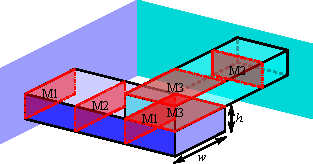
\includegraphics[width=.75\columnwidth]{sources/method/failure_modes_diagonal.pdf}
	\caption{Failure can happen when either beam shears off completely (M1), when both beams break in one location (M2) or at the interface between the two (M3).}
	\label{fig:failure_modes_diagonal}
\end{figure}









Maybe the pattern does perform better in a non-45 degree angle!
Can we force the fingers to be tensile-prone, but the beams to be shear-prone?











\subsection{Orientation}
According to experimental results the diagonal orientation outperforms the axis aligned one.
See \cref{graph:45vs90}.
Tensile tests were performed on $14.6\times15\times100$\si{\milli\meter} bars of Ultimaker green Tough PLA and Ultimaker transparent PP
printed on an Ultimaker S5 at a default layer height profile of \SI{0.1}{\milli\meter} with an adjusted infill density of \SI{80}{\percent}
on an Instron 3366 Universal Testing machine at \SI{5}{\milli\meter\per\minute}.
The structures consisted of beams with a constant width of twice the outer wall line width, i.e. \SI{0.7}{\milli\meter} and \SI{0.76}{\milli\meter} for TPLA and PP respectively,
oriented at \SI{90}{\degree} and \SI{45}{\degree} w.r.t the tensile force.

\begin{figure}
	\centering
	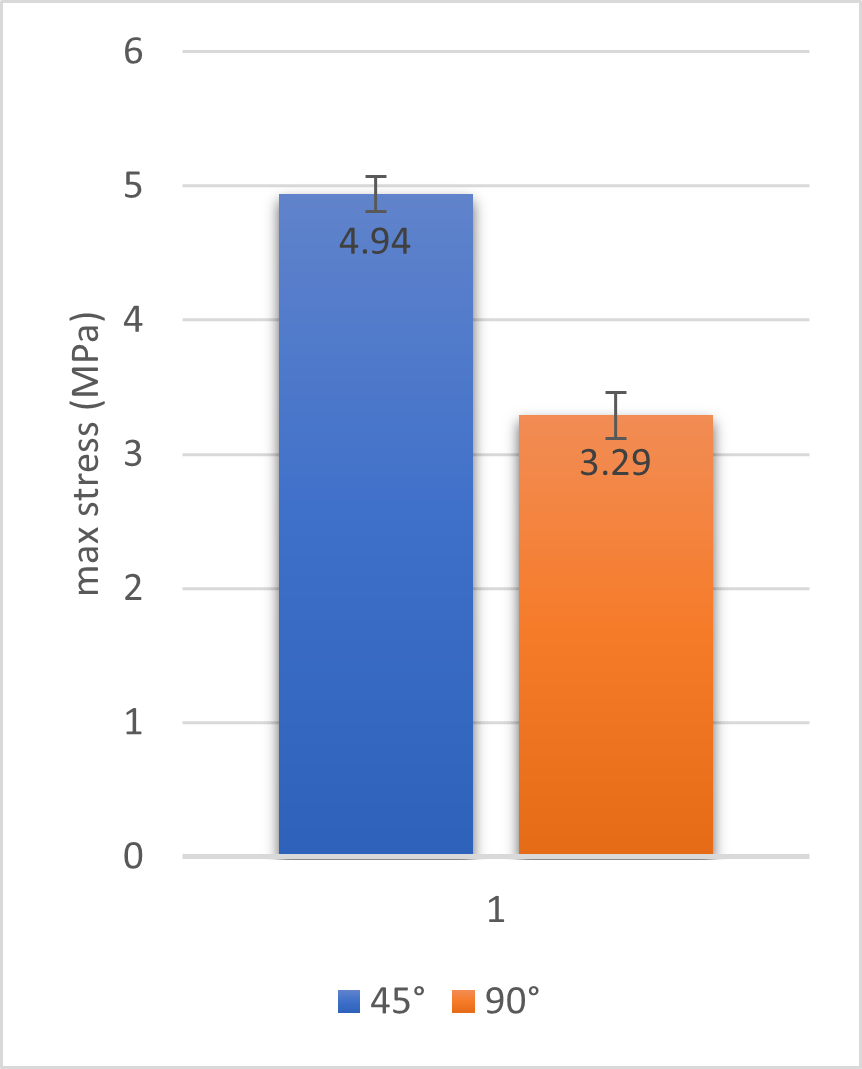
\includegraphics[width=.5\columnwidth]{sources/testing/45vs90.png}
	\caption{Impact of pattern orientation.}
	\label{graph:45vs90}
\end{figure}


\begin{figure}
	\centering
	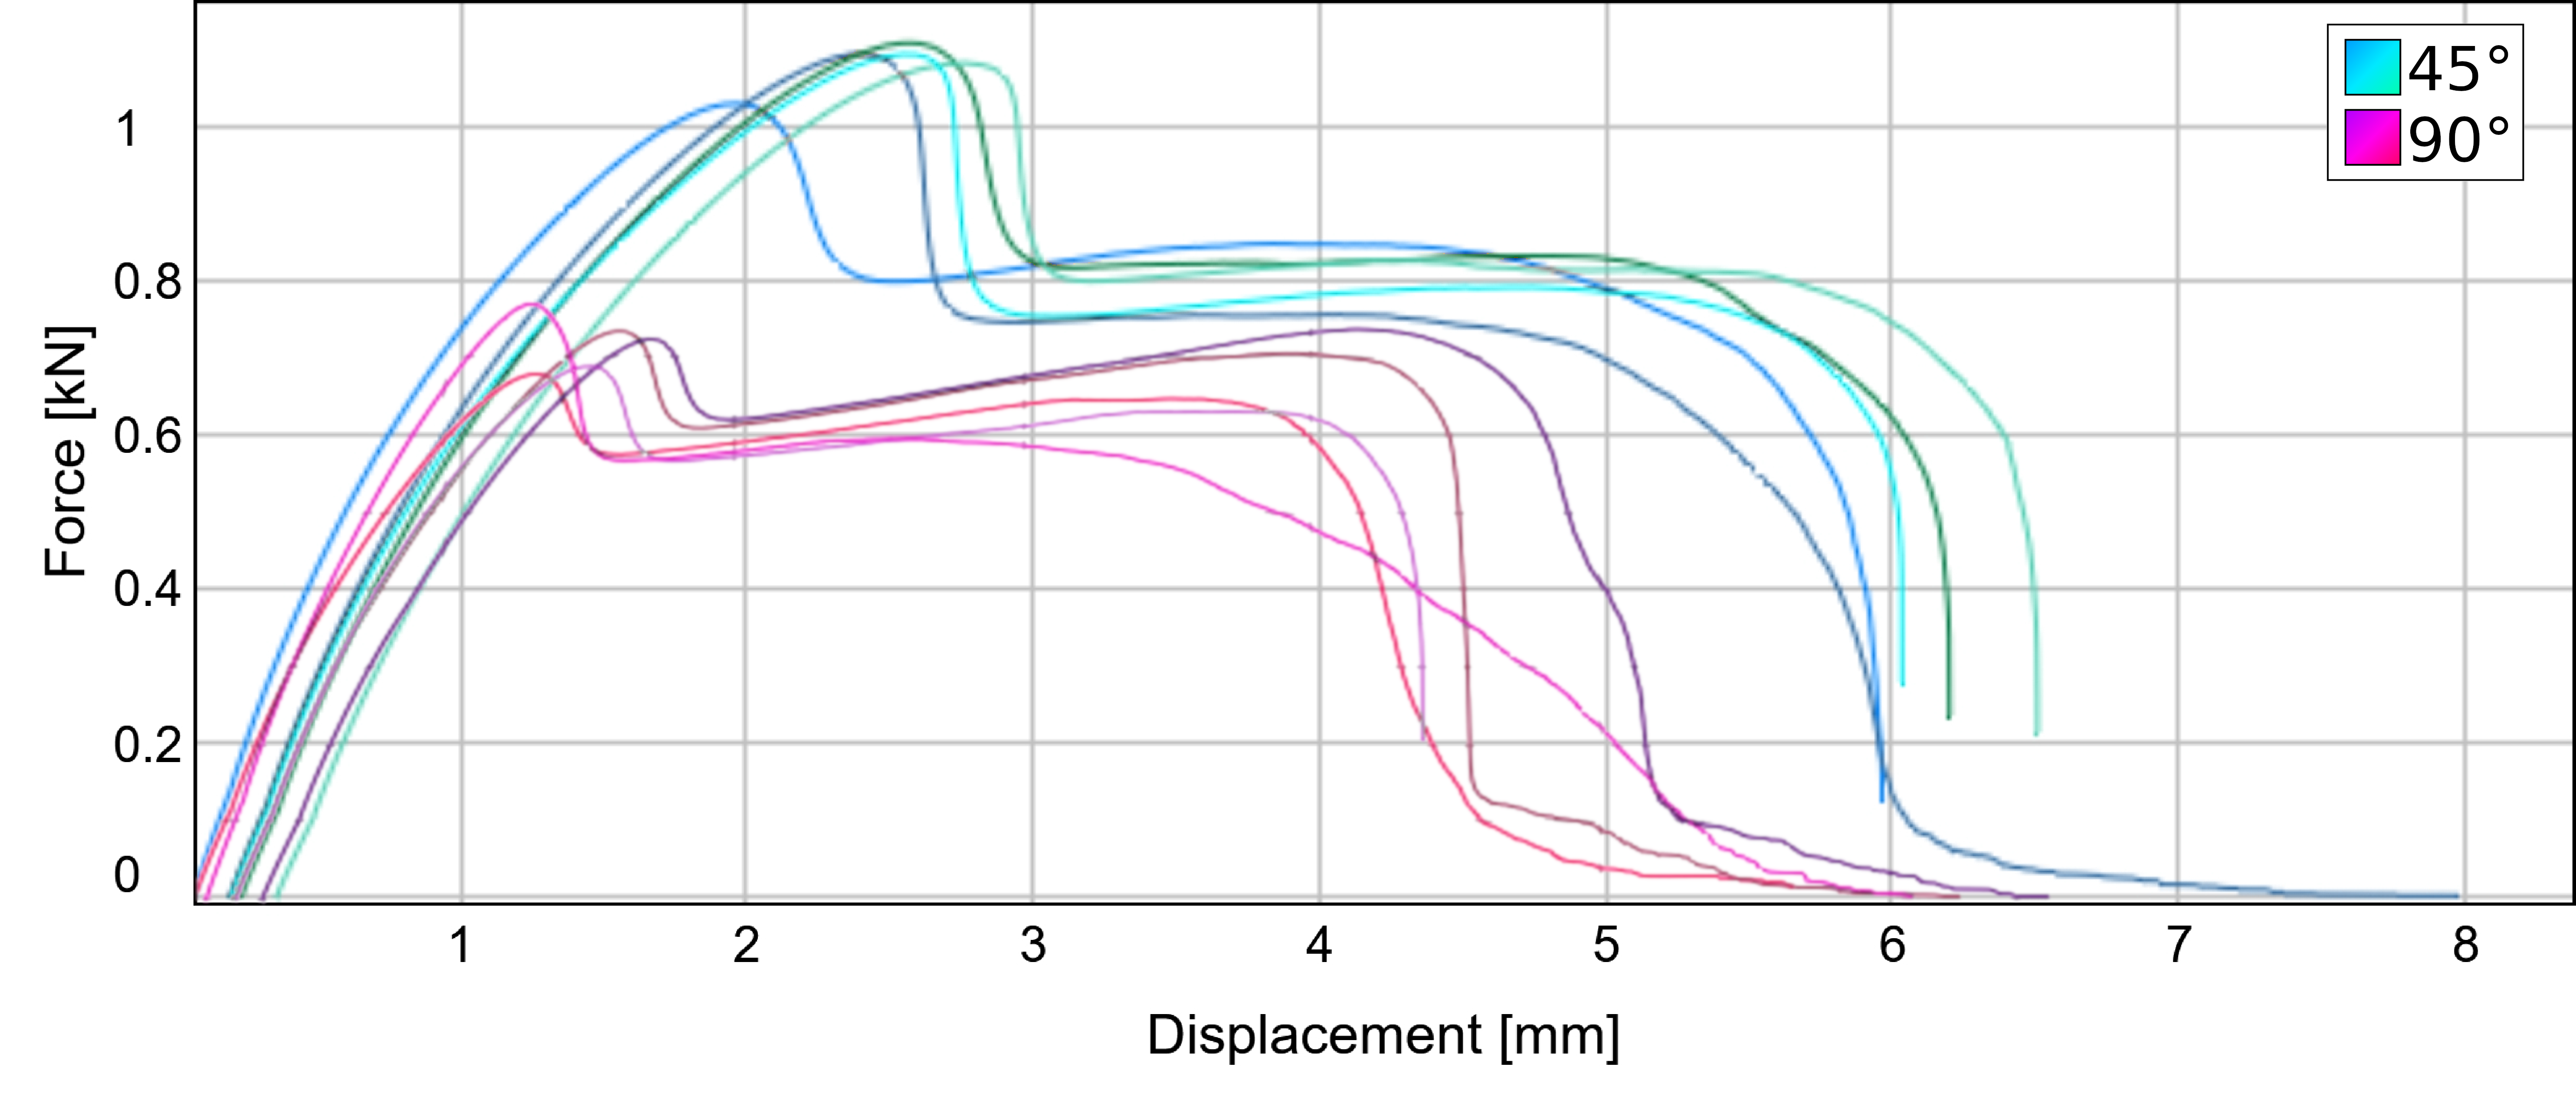
\includegraphics[width=\columnwidth]{sources/testing/45vs90_stress_strain.png}
	\caption{Impact of pattern orientation.}
	\label{graph:45vs90_stress_strain}
\end{figure}
